
%----------------------------------------------------------------------------------------
%	PACKAGES AND THEMES
%----------------------------------------------------------------------------------------

\documentclass{beamer}

\usetheme{Warsaw}

\usepackage{listings}
\usepackage{graphicx}
\usepackage[utf8]{inputenc}
\usepackage{url}
\setbeamertemplate{itemize item}[triangle]
%----------------------------------------------------------------------------------------
%	TITLE PAGE
%----------------------------------------------------------------------------------------

\title{Design patterns} % The short title appears at the bottom of every slide, the full title is only on the title page

\author{Venkatesh} % Your name
\institute{WDC}
\date{\today} % Date, can be changed to a custom date

\begin{document}

\lstset{
    basicstyle=\ttfamily\footnotesize,
    breaklines=true
    breakatwhitespace=true,
    language=C++,
    columns=fullflexible,
    keepspaces=true,
    breaklines=true,
    tabsize=3, 
    showstringspaces=false,
    extendedchars=true
    inputencoding=utf8
}

\begin{frame}
\titlepage % Print the title page as the first slide
\end{frame}

\begin{frame}{Outline}
  % You might wish to add the option [pausesections]
  \begin{enumerate}
   \item Structural Patterns
        \begin{itemize}
        \item Adapter
        \item Bridge
        \item Proxy
        \end{itemize}
   \item Behavioral Patterns
        \begin{itemize}
        \item Mediator
        \item Memento
        \end{itemize}
  \end{enumerate}
\end{frame}


%----------------------------------------------------------------------------------------
%	PRESENTATION SLIDES
%----------------------------------------------------------------------------------------

%----------------------------------------------------------------------------------------

\begin{frame}[fragile]
\frametitle{Structural Patterns}

\begin{itemize}
\item Responsible for building simple and efficient class hierarchies and relations between different classes
\item Class patterns use inheritance
\item Object patterns use \texttt{object composition}

\end{itemize}

\end{frame}

\begin{frame}[fragile]
\frametitle{Adapter}

\begin{itemize}
\item Also known as \texttt{Wrapper}
\item Used to make existing classes work with others without modifying their source code
\end{itemize}

\end{frame}

\begin{frame}[fragile]
\frametitle{Adapter ...}

\begin{block}{solves problems like:}
    How can a class be reused that does not have an interface that a client requires?
\end{block}

\end{frame}

\begin{frame}[fragile]
\frametitle{Adapter ...}

\begin{block}{how to solve:}
    Define a separate Adapter class that converts the (incompatible) 
    interface of a class (Adaptee) into another interface (Target) clients require.
\end{block}

\end{frame}


\begin{frame}[fragile]
\frametitle{Adapter ...}
There are two ways to define an Adapter:
\begin{itemize}
    \item \texttt{Class Adapter} : Uses inheritance to implement Target Interface
    \item \texttt{Object Adapter} : Uses object composition to implement Target Interface
\end{itemize}

\begin{block}{Note:} 
Adapter is responsible for functionality the adapted class doesn't provide
\end{block}

\end{frame}


\begin{frame}[fragile]
\frametitle{Structure}

 \begin{figure}[ht]
       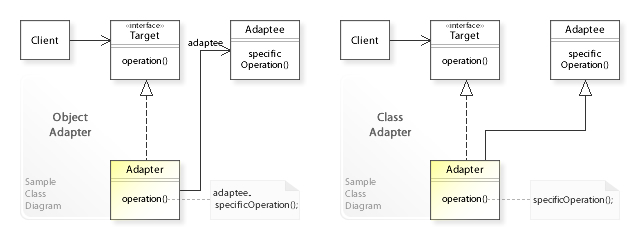
\includegraphics[width=11cm]{./images/adapter.jpg}
 \end{figure}

\end{frame}

\begin{frame}[fragile]
\frametitle{Sample Code}
    
\end{frame}

\begin{frame}[fragile]
\frametitle{Class adapter vs Object adapter}
\begin{block}{class adapter}
    \begin{itemize}
    \item adapts Adaptee to Target by commiting to a concrete Adapter class
         \begin{itemize}
            \item It won't work, if we want to adapt a class and all its subclasses 
        \end{itemize}
     \item lets Adapter override some of Adaptee's behavior
     \item no additional pointer indirection is needed
    \end{itemize}
\end{block}

\end{frame}

\begin{frame}[fragile]
\frametitle{Class adapter vs Object adapter}
\begin{block}{object adapter}
    \begin{itemize}
    \item lets a single Adapter work with many Adaptees - Adaptee itself and all of its subclasses
     \item harder to override Adaptee behavior
    \end{itemize}
\end{block}

\end{frame}


\begin{frame}[fragile]
\frametitle{Bridge}

\begin{itemize}
\item Also Known as \texttt{"Handle/Body"}
\item "Decouple an abstraction from its implementation so that the two can vary independently"
\end{itemize}

\end{frame}

\begin{frame}[fragile]
\frametitle{Bridge ...}

\begin{block}{solves problems like:}
    A compile-time binding between an abstraction and its implementation should be 
    avoided so that an implementation can be selected at run-time.
\end{block}

\end{frame}

\begin{frame}[fragile]
\frametitle{Bridge ...}

\begin{block}{how to solve:}
    \begin{itemize}
    \item Separate an abstraction (Abstraction) from its implementation (Implementor) by putting them in separate class hierarchies
    \item Implement the Abstraction in terms of (by delegating to) an Implementor object
    \end{itemize}
\end{block}

\end{frame}


\begin{frame}[fragile]
\frametitle{Structure}

 \begin{figure}[ht]
       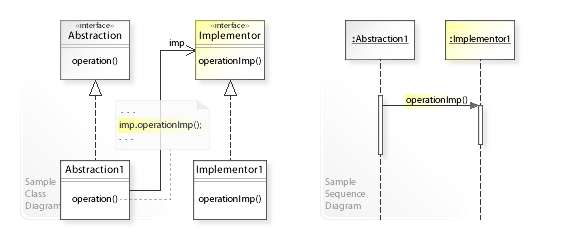
\includegraphics[width=11cm]{./images/Bridge.jpg}
 \end{figure}

\end{frame}


\begin{frame}[fragile]
\frametitle{Sample Code}

\end{frame}



\begin{frame}[fragile]
\frametitle{Proxy}

\begin{itemize}
\item Also known as \texttt{Surrogate}
\item Provide a surrogate or placeholder for another object to control access to it
\end{itemize}

\end{frame}

\begin{frame}[fragile]
\frametitle{Proxy ...}

\begin{block}{solves problems like:}

\begin{itemize}
\item How can the access to an object be controlled?
\item How can additional functionality be provided when accessing an object?
\end{itemize}

\end{block}

\end{frame}

\begin{frame}[fragile]
\frametitle{Proxy ...}

\begin{block}{how to solve:}
Define a separate Proxy object that
\begin{itemize}
\item can be used as substitute for another object (Subject)
\item Work through a Proxy object to control the access to an object
\end{itemize}
\end{block}

\end{frame}



\begin{frame}[fragile]
\frametitle{Proxy...}
\begin{block}{Common Kinds of Proxies}
\begin{itemize}
\item remote proxy  : hide complex network communication details
\item virtual proxy : defer expensive objects creation until needed
\item protection proxy : check access rights for sensitive objects
\item smart reference : performs additional actions when object is accessed
\end{itemize}
\end{block}

\end{frame}

\begin{frame}[fragile]
\frametitle{Structure}

 \begin{figure}[ht]
       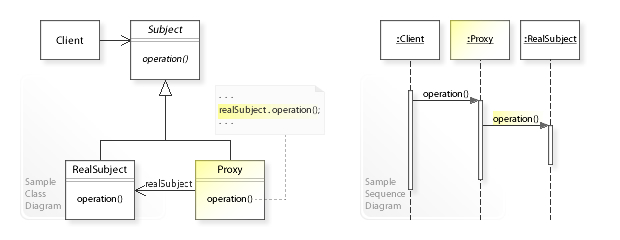
\includegraphics[width=11cm]{./images/proxy.jpg}
 \end{figure}

\end{frame}




\begin{frame}[fragile]
\frametitle{Sample Code}

\end{frame}


\begin{frame}[fragile]
\frametitle{Adapter vs Proxy}

\begin{itemize}
\item An Adapter provides a different interface to the object it adapts
\item A proxy provides the same interface as its subject
\end{itemize}

\end{frame}


\begin{frame}[fragile]
\frametitle{Adapter vs Bridge}
\begin{itemize}
\item Adapter pattern is applied to systems \texttt{after they're designed}
\item Bridge is used \texttt{up-front in design} to let abstractions and implementations vary independently
\end{itemize}
\end{frame}



\begin{frame}[fragile]
\frametitle{Behavioral Patterns}

\begin{itemize}
\item Concerned with 
    \begin{itemize}
    \item algorithms 
    \item assignment of responsibilities between objects
    \item communication between objects 
    \end{itemize}
\end{itemize}

\end{frame}




\begin{frame}[fragile]
\frametitle{Mediator}
\begin{itemize}
\item Define an object that encapsulates how a set of objects interact
\item Objects no longer communicate directly with each other 
    \begin{itemize}
        \item instead communicate through the mediator
    \end{itemize}     
\end{itemize}
\end{frame}


\begin{frame}[fragile]
\frametitle{Mediator ...}

\begin{block}{solves problems like:}
\begin{itemize}
\item How can tight coupling between a set of interacting objects be avoided? 
\item How can the interaction between a set of objects be changed independently? 
\end{itemize}
\end{block}

\end{frame}

\begin{frame}[fragile]
\frametitle{Mediator ...}

\begin{block}{how to solve:}
\begin{itemize}
    \item Define a separate (mediator) object that encapsulates the interaction between a set of objects
    \item Objects delegate their interaction to a mediator object 
        \begin{itemize}
            \item instead of interacting with each other directly
        \end{itemize}
\end{itemize}
\end{block}

\end{frame}


\begin{frame}[fragile]
\frametitle{Mediator ...}

\begin{block}{Consequences}

\begin{itemize}
\item It decouples colleagues : promotes loose coupling between colleagues
\item It centralizes control  : makes the mediator itself a monolith
\end{itemize}

\end{block}

\end{frame}


\begin{frame}[fragile]
\frametitle{Structure}

 \begin{figure}[ht]
       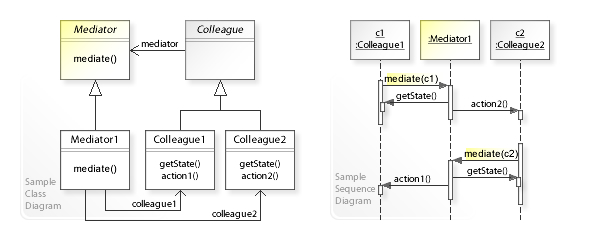
\includegraphics[width=11cm]{./images/mediator.jpg}
 \end{figure}

\end{frame}


\begin{frame}[fragile]
\frametitle{Sample Code}
    
\end{frame}



\begin{frame}[fragile]
\frametitle{Memento}

\begin{itemize}
\item Provides the ability to restore an object to its previous state (undo)

\end{itemize}

\end{frame}


\begin{frame}[fragile]
\frametitle{Memento ...}

\begin{block}{solves problems like:}
    \begin{itemize}
        \item Without violating encapsulation,
        \item internal state of an object should be saved externally so that the object can be restored to this state later
    \end{itemize}
\end{block}

\end{frame}

\begin{frame}[fragile]
\frametitle{Memento ...}

\begin{block}{how to solve:}
Make an object (originator) itself responsible for
    \begin{itemize}
    \item saving its internal state to a (memento) object and
    \item restoring to a previous state from a (memento) object
    \item only the originator is allowed to access a memento 
    \end{itemize}
\end{block}

\end{frame}


\begin{frame}[fragile]
\frametitle{Memento ...}

\begin{block}{Usage}
\begin{itemize}
\item A client (caretaker) can request a memento from the originator 
(to save the internal state of the originator)
\item A client can pass a memento back to the originator (to restore to a previous state)
\item Caretaker is responsible for deleting the mementos it cares for
\end{itemize}
\end{block}

\end{frame}


\begin{frame}[fragile]
\frametitle{Structure}

 \begin{figure}[ht]
       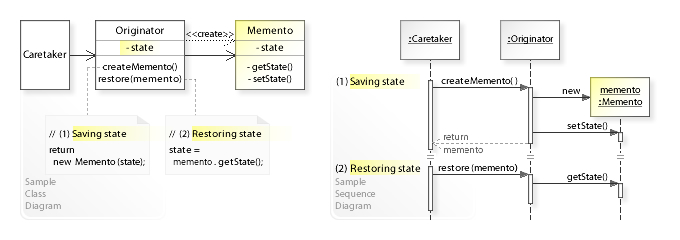
\includegraphics[width=11cm]{./images/memento.jpg}
 \end{figure}

\end{frame}

\begin{frame}[fragile]
\frametitle{Memento ...}

\begin{block}{Consequences}
    \begin{itemize}
    \item Using mementos might be expensive : copy large amount of information
    \item Defining narrow and wide interfaces : difficult in some languages 
    \end{itemize}
\end{block}

\end{frame}



\begin{frame}[fragile]
\frametitle{Sample Code}
    
    \begin{columns}
    \begin{column}{0.48\textwidth}
    \begin{lstlisting}
class State;
class Memento;

class Originator {
public:
    Memento* CreateMemento();
    void restore(const Memento *);
    // ..
private:
    // internal data structures
    State* _state;
    // ...
};
    \end{lstlisting}
    \end{column}
    \begin{column}{0.48\textwidth}
    \begin{lstlisting}
class Memento {
public:
// narrow public interface
    virtual ~Memento();
private:
    friend class Originator;
    Memento(State *);
    State * getState();
    // ...
private:
    State * _state;
    // ...
};
    \end{lstlisting}
    \end{column}
\end{columns}
    
\end{frame}


%------------------------------------------------
\begin{frame}
\frametitle{References}
\begin{thebibliography}{2} % Beamer does not support BibTeX so references must be inserted manually as below
\setbeamertemplate{bibliography item}[book]
\bibitem{GoF} Design Patterns - Erich Gamma, Richard helm, Ralph Johnson, John Vlissides
\end{thebibliography}
\end{frame}

%------------------------------------------------

\begin{frame}
\Huge{\centerline{Thank You}}
\end{frame}

%----------------------------------------------------------------------------------------




%----------------------------------------------------------------------------------------

\end{document} 

